\documentclass[12pt,a4paper]{article}
\usepackage[a4paper,top=12mm,bottom=12mm,left=15mm,right=15mm]{geometry}
\usepackage[T1]{fontenc}
\usepackage{amsmath}
\usepackage{amssymb}
\usepackage{tgadventor}
\renewcommand*{\familydefault}{\sfdefault}
\usepackage[italic]{mathastext}
\usepackage{enumitem}
\usepackage{xcolor}
\usepackage{tikz}
\usetikzlibrary{calc}
\usepackage[most]{tcolorbox}

\pagestyle{empty}
\setlength{\parindent}{0pt}
\setlength{\parskip}{4pt}
\AtBeginDocument{\raggedright}
\hyphenpenalty=10000
\exhyphenpenalty=10000
\setlist[enumerate]{label=(\alph*), leftmargin=*, itemsep=4pt, topsep=2pt}
\setlist[itemize]{leftmargin=*, itemsep=2pt, topsep=2pt}

\newtcolorbox{solbox}[1][]{breakable,colback=blue!3,colframe=blue!35,
  boxrule=0.5pt,left=6pt,right=6pt,top=5pt,bottom=5pt,#1}

\newcounter{sol}
\newcommand{\s}{\refstepcounter{sol}\textbf{Q\thesol.}\ }
\newcommand{\ans}[1]{\par\smallskip\noindent\textbf{Answer:} #1\par}
\newcommand{\pt}[3]{\fill #1 circle (1.5pt); \node[inner sep=2pt,#2] at #1 {$#3$};}
\newcommand{\place}[3]{\fill #1 circle (1.5pt); \node[inner sep=2pt,#2] at #1 {#3};}

\tikzset{
  given/.style={line width=0.8pt},
  construction/.style={line width=0.5pt, blue!70},
  locus/.style={line width=0.8pt, red!70, dashed},
}

\begin{document}

\begin{center}
  {\LARGE\bfseries Constructions and Loci}\\[3pt]
  {\Large Worked Solutions}
\end{center}

\vspace{2pt}
\textit{Measurements are approximate: accept answers within about 1\,mm. The diagrams show the final construction or locus; the important point is the position of the constructed line or region.}

\section*{A. Constructions (Q1--Q7)}

\s Construct the perpendicular bisector of the line segment \(AB\).

\begin{solbox}
Open the compasses to more than half of \(AB\). Draw arcs with centre \(A\) and with centre \(B\), crossing above and below \(AB\). Join the two crossing points. The joining line is the perpendicular bisector of \(AB\). Since \(AB=8\)\,cm, it crosses \(AB\) at its midpoint, \(4\)\,cm from \(A\) and \(4\)\,cm from \(B\).
\end{solbox}

\begin{center}
\begin{tikzpicture}[scale=0.8]
  \useasboundingbox (-1,-4) rectangle (9,4);
  \draw[given] (0,0) -- (8,0);
  \draw[construction] (0,0) ++(36.87:5) arc (36.87:-36.87:5);
  \draw[construction] (8,0) ++(143.13:5) arc (143.13:216.87:5);
  \draw[locus] (4,-3.5) -- (4,3.5);
  \fill (4,0) circle (1.5pt);
  \node[below] at (0,0) {\(A\)};
  \node[below] at (8,0) {\(B\)};
  \node[right] at (4,0) {midpoint};
\end{tikzpicture}
\end{center}

\s Construct the perpendicular from the point \(P\) to the line. Then measure the distance from \(P\) to the line.

\begin{solbox}
Draw an arc with centre \(P\) to cut the line twice. Construct the perpendicular bisector of the two cut points; this line passes through \(P\) and is perpendicular to the given line. The foot of the perpendicular is \(8\)\,cm from the left-hand end, and the perpendicular distance is \(3\)\,cm.
\end{solbox}
\ans{\(3\)\,cm}

\begin{center}
\begin{tikzpicture}[scale=0.75]
  \useasboundingbox (-0.5,-2) rectangle (13.5,4);
  \draw[given] (0,0) -- (13,0);
  \draw[construction] (8,3) ++(-131.41:4) arc (-131.41:-48.59:4);
  \draw[locus] (8,0) -- (8,3);
  \draw (8,0) rectangle (8.4,0.4);
  \pt{(8,3)}{above}{P}
\end{tikzpicture}
\end{center}

\s Construct the perpendicular to the line at the point \(Q\).

\begin{solbox}
With centre \(Q\), mark equal lengths on the line on either side of \(Q\). Draw equal arcs from these two marks so that they cross above and below the line. Join \(Q\) to a crossing point. The line through \(Q\) at right angles to the given line is the required perpendicular.
\end{solbox}

\begin{center}
\begin{tikzpicture}[scale=0.75]
  \useasboundingbox (-0.5,-2) rectangle (13,2.5);
  \draw[given] (0,0) -- (13,0);
  \draw[construction] (3.5,0) ++(48.2:1.5) arc (48.2:-48.2:1.5);
  \draw[construction] (5.5,0) ++(131.8:1.5) arc (131.8:228.2:1.5);
  \draw[locus] (4.5,-1.5) -- (4.5,1.5);
  \draw (4.5,0) rectangle (4.9,0.4);
  \pt{(4.5,0)}{below}{Q}
\end{tikzpicture}
\end{center}

\newpage

\s Construct the perpendicular from the point \(R\) to the line. Then measure the distance from \(R\) to the line.

\begin{solbox}
The perpendicular from \(R\) meets the line at the foot of the perpendicular. Measuring along this perpendicular gives \(3\)\,cm.
\end{solbox}
\ans{\(3\)\,cm}

\begin{center}
\begin{tikzpicture}[scale=0.8]
  \useasboundingbox (-0.5,-2) rectangle (13,5);
  \begin{scope}[rotate=20]
    \draw[given] (0,0) -- (12.5,0);
    \draw[locus] (6.5,0) -- (6.5,-3);
    \draw (6.5,0) -- (6.5,-0.4) -- (6.9,-0.4) -- (6.9,0) -- cycle;
    \pt{(6.5,-3)}{below}{R}
  \end{scope}
\end{tikzpicture}
\end{center}

\s Construct the perpendicular bisector of the line segment \(CD\). Mark the midpoint \(M\) of \(CD\), and measure the length of \(CM\).

\begin{solbox}
The construction gives the perpendicular bisector of \(CD\). It crosses \(CD\) at its midpoint \(M\). Since \(CD=7\)\,cm,
\[
CM=MD=\frac{7}{2}=3.5\text{ cm}.
\]
\end{solbox}
\ans{\(3.5\)\,cm}

\begin{center}
\begin{tikzpicture}[scale=0.85]
  \useasboundingbox (-3.5,-3.5) rectangle (3.5,3.5);
  \begin{scope}[rotate=40]
    \draw[given] (-3.5,0) -- (3.5,0);
    \draw[locus] (0,-3) -- (0,3);
    \fill (0,0) circle (1.5pt);
    \node[below] at (-3.5,0) {\(C\)};
    \node[above] at (3.5,0) {\(D\)};
    \node[below left] at (0,0) {\(M\)};
  \end{scope}
\end{tikzpicture}
\end{center}

\s Construct the perpendicular to the line at the point \(S\).

\begin{solbox}
The given line is vertical. A line perpendicular to it is horizontal. So the perpendicular at \(S\) is the horizontal line through \(S\).
\end{solbox}

\begin{center}
\begin{tikzpicture}[scale=0.8]
  \useasboundingbox (-3.5,-3.5) rectangle (3.5,3.5);
  \draw[given] (-1.2,-3.3) -- (-1.2,3.3);
  \draw[locus] (-3.3,-0.6) -- (3.3,-0.6);
  \draw (-1.2,-0.6) rectangle (-0.8,-0.2);
  \pt{(-1.2,-0.6)}{left}{S}
\end{tikzpicture}
\end{center}

\s
\begin{enumerate}
  \item Construct the perpendicular from the point \(G\) to the line.
  \item Construct the perpendicular to the line at the point \(H\).
  \item What do you notice about your two perpendiculars?
\end{enumerate}

\begin{solbox}
(a) Drop the perpendicular from \(G\) to the line. (b) Draw the perpendicular to the line at \(H\). (c) Both constructed lines are perpendicular to the same straight line, so they are parallel to each other.
\end{solbox}
\ans{They are parallel.}

\begin{center}
\begin{tikzpicture}[scale=0.75]
  \useasboundingbox (-0.5,-3) rectangle (14,4);
  \draw[given] (0,0) -- (13.5,0);
  \draw[locus] (3,0) -- (3,2.5);
  \draw[locus] (9.5,-1.5) -- (9.5,3.5);
  \draw (3,0) rectangle (3.4,0.4);
  \draw (9.5,0) rectangle (9.9,0.4);
  \pt{(3,2.5)}{above}{G}
  \pt{(9.5,0)}{below}{H}
\end{tikzpicture}
\end{center}

\newpage

\section*{B. Using the constructions (Q8--Q10)}

\s The diagram shows the triangle \(ABC\).
\begin{enumerate}
  \item Construct the perpendicular from \(C\) to the line segment \(AB\).
  \item The perpendicular from \(C\) to \(AB\) is the height of the triangle. Measure the height.
  \item The base \(AB\) is \(7\)\,cm long. Work out the area of the triangle \(ABC\).
\end{enumerate}

\begin{solbox}
(a) The perpendicular from \(C\) meets \(AB\) at the foot of the altitude. In this diagram the foot is \(2\)\,cm from \(A\). (b) The height is \(4\)\,cm. (c) 
\[
\text{Area}=\frac12\times AB\times \text{height}
=\frac12\times 7\times 4=14\text{ cm}^2.
\]
\end{solbox}
\ans{(b) \(4\)\,cm \qquad (c) \(14\)\,cm\(^2\)}

\begin{center}
\begin{tikzpicture}[scale=0.9]
  \useasboundingbox (-0.8,-0.8) rectangle (7.8,4.6);
  \draw[given, line join=round] (0,0) -- (7,0) -- (2,4) -- cycle;
  \draw[locus] (2,0) -- (2,4);
  \draw (2,0) rectangle (2.35,0.35);
  \pt{(0,0)}{below left}{A}
  \pt{(7,0)}{below right}{B}
  \pt{(2,4)}{above}{C}
\end{tikzpicture}
\end{center}

\s The points \(E\) and \(F\) are on the line, \(4\)\,cm apart.
\begin{enumerate}
  \item Construct the perpendicular to the line at \(E\), and the perpendicular to the line at \(F\).
  \item Use your compasses to mark the point \(G\) on the perpendicular at \(F\), and the point \(H\) on the perpendicular at \(E\), so that \(EFGH\) is a square.
  \item Measure the diagonal \(EG\).
\end{enumerate}

\begin{solbox}
(a) Draw the perpendiculars at \(E\) and at \(F\). (b) Mark \(G\) and \(H\) \(4\)\,cm from the line, so that \(EFGH\) has four equal sides and four right angles. (c) The diagonal of a square of side \(4\)\,cm is
\[
EG=\sqrt{4^2+4^2}=4\sqrt2\approx 5.66\text{ cm}.
\]
So the measured diagonal is about \(5.7\)\,cm.
\end{solbox}
\ans{\(5.7\)\,cm (about \(5.66\)\,cm)}

\begin{center}
\begin{tikzpicture}[scale=0.8]
  \useasboundingbox (-2.4,-0.9) rectangle (6.4,5.1);
  \draw[given] (-2.2,0) -- (6.2,0);
  \draw[locus] (0,0) -- (0,4);
  \draw[locus] (4,0) -- (4,4);
  \draw[given] (0,4) -- (4,4);
  \draw[given] (0,0) -- (4,4);
  \pt{(0,0)}{below}{E}
  \pt{(4,0)}{below}{F}
  \pt{(4,4)}{above}{G}
  \pt{(0,4)}{above}{H}
\end{tikzpicture}
\end{center}

\newpage

\s A \textbf{chord} is a line segment that joins two points on a circle. The centre of this circle has not been marked.
\begin{enumerate}
  \item Construct the perpendicular bisector of the chord \(PQ\).
  \item Construct the perpendicular bisector of the chord \(RS\).
  \item The centre of the circle is the point where your two perpendicular bisectors cross. Mark it, and label it \(O\).
  \item Measure the radius of the circle.
  \item Set your compasses to this radius, and draw a circle with centre \(O\). Your circle should lie on top of the circle that is drawn.
\end{enumerate}

\begin{solbox}
The perpendicular bisector of any chord passes through the centre of the circle. The two perpendicular bisectors therefore meet at the centre \(O\). Measuring from \(O\) to the drawn circle gives a radius of \(3.5\)\,cm.
\end{solbox}
\ans{\(3.5\)\,cm}

\begin{center}
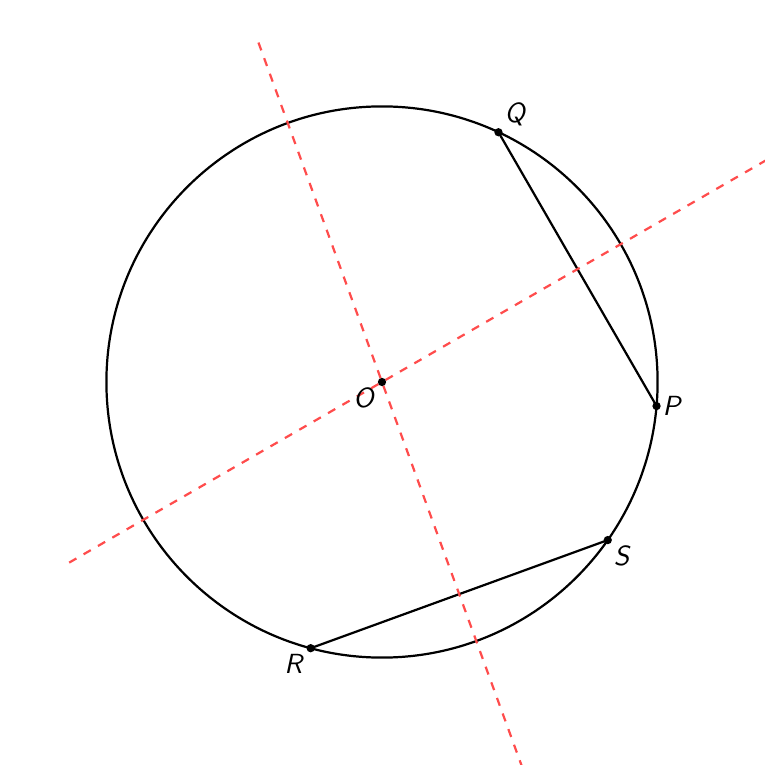
\begin{tikzpicture}[scale=1.0]
  \useasboundingbox (-4.5,-4.5) rectangle (4.5,4.5);
  \coordinate (O) at (0,0);
  \coordinate (P) at (355:3.5);
  \coordinate (Q) at (65:3.5);
  \coordinate (R) at (255:3.5);
  \coordinate (S) at (325:3.5);
  \coordinate (mPQ) at ($(P)!0.5!(Q)$);
  \coordinate (mRS) at ($(R)!0.5!(S)$);
  \draw[given] (O) circle (3.5);
  \draw[given] (P) -- (Q);
  \draw[given] (R) -- (S);
  \draw[locus] ($(O)!-1.6!(mPQ)$) -- ($(O)!2.2!(mPQ)$);
  \draw[locus] ($(O)!-1.6!(mRS)$) -- ($(O)!2.2!(mRS)$);
  \pt{(P)}{right}{P}
  \pt{(Q)}{above right}{Q}
  \pt{(R)}{below left}{R}
  \pt{(S)}{below right}{S}
  \pt{(O)}{below left}{O}
\end{tikzpicture}
\end{center}

\newpage

\section*{C. Loci (Q11--Q14)}

\s The rule for this locus is that the point is \(3\)\,cm from \(C\).
\begin{enumerate}
  \item Use your ruler to mark \(8\) points that are \(3\)\,cm from \(C\).
  \item What shape do your points make?
  \item Use your compasses to draw the locus of the points that are \(3\)\,cm from \(C\).
  \item Shade the region of the points that are less than \(3\)\,cm from \(C\).
\end{enumerate}

\begin{solbox}
(a) The marked points lie on a circle of radius \(3\)\,cm centred at \(C\). (b) They make a circle. (c) Draw the circle with centre \(C\) and radius \(3\)\,cm. (d) The points less than \(3\)\,cm from \(C\) fill the inside of this circle; shade that region.
\end{solbox}
\ans{(b) A circle.}

\begin{center}
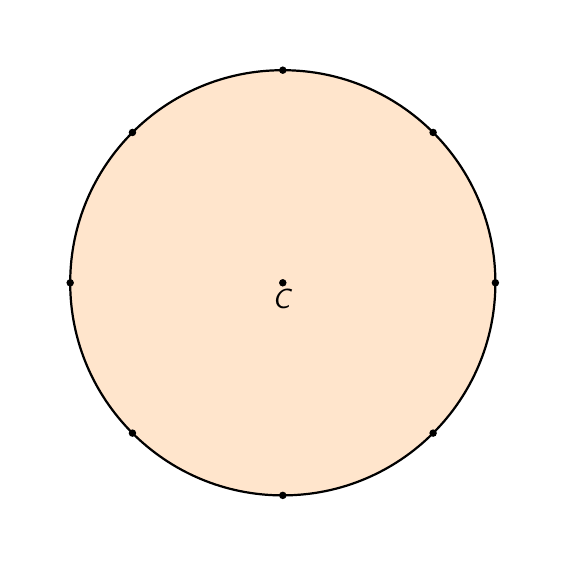
\begin{tikzpicture}[scale=0.9]
  \useasboundingbox (-3.6,-3.6) rectangle (3.6,3.6);
  \fill[orange!20] (0,0) circle (3);
  \draw[given] (0,0) circle (3);
  \foreach \a in {0,45,90,135,180,225,270,315}
    \fill (\a:3) circle (1.5pt);
  \pt{(0,0)}{below}{C}
\end{tikzpicture}
\end{center}

\s A point is \textbf{equidistant} from \(A\) and \(B\) when it is the same distance from \(A\) as it is from \(B\).
\begin{enumerate}
  \item Set your compasses to \(4\)\,cm. Draw arcs with centres \(A\) and \(B\), crossing above and below \(AB\). Mark the two crossing points.
  \item Do the same with your compasses set to \(5\)\,cm.
  \item Mark the point on the line segment \(AB\) that is equidistant from \(A\) and \(B\).
  \item Draw the straight line through your points. Which construction draws this line?
  \item Shade the region of the points that are closer to \(A\) than to \(B\).
\end{enumerate}

\begin{solbox}
With \(AB=6\)\,cm, the midpoint is \(3\)\,cm from \(A\) and from \(B\). The \(4\)\,cm arcs cross at points \(3\)\,cm horizontally from the midpoint and
\[
\sqrt{4^2-3^2}=\sqrt7\approx 2.65\text{ cm}
\]
above and below \(AB\). The \(5\)\,cm arcs cross \(\sqrt{5^2-3^2}=4\)\,cm above and below \(AB\). The line through these points is the perpendicular bisector of \(AB\). The points closer to \(A\) are on \(A\)'s side of this line, so shade that half-plane.
\end{solbox}
\ans{(d) The perpendicular bisector of \(AB\).}

\begin{center}
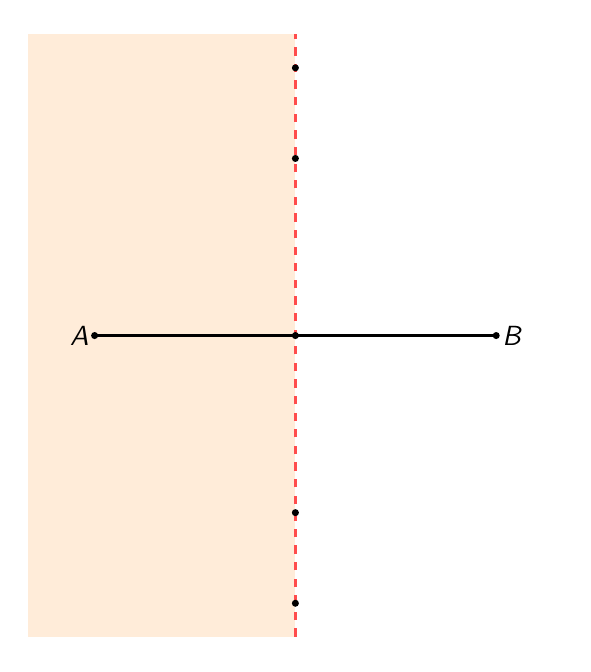
\begin{tikzpicture}[scale=0.85]
  \useasboundingbox (-1,-4.6) rectangle (7,4.6);
  \fill[orange!15] (-1,-4.5) rectangle (3,4.5);
  \draw[given] (0,0) -- (6,0);
  \draw[locus] (3,-4.5) -- (3,4.5);
  \fill (3,2.6458) circle (1.5pt);
  \fill (3,-2.6458) circle (1.5pt);
  \fill (3,4) circle (1.5pt);
  \fill (3,-4) circle (1.5pt);
  \fill (3,0) circle (1.5pt);
  \pt{(0,0)}{left}{A}
  \pt{(6,0)}{right}{B}
\end{tikzpicture}
\end{center}

\newpage

\s The map shows two lighthouses, \(L\) and \(M\). The scale is \(1\)\,cm to \(2\)\,km. A boat is less than \(7\)\,km from \(L\), and closer to \(M\) than to \(L\).
\begin{enumerate}
  \item How many centimetres on the map is \(7\)\,km?
  \item Draw the locus of the points that are \(7\)\,km from \(L\).
  \item Construct the locus of the points that are equidistant from \(L\) and \(M\).
  \item Shade the region where the boat could be.
\end{enumerate}

\begin{solbox}
(a) \(7\)\,km represents
\[
7\div 2=3.5\text{ cm}
\]
on the map. (b) Draw the circle with centre \(L\) and radius \(3.5\)\,cm. (c) Construct the perpendicular bisector of \(LM\). It crosses \(LM\) at its midpoint, about \(2.3\)\,cm from \(L\). (d) The boat is inside the circle and on \(M\)'s side of the perpendicular bisector; shade the part of the inside of the circle that is closer to \(M\).
\end{solbox}
\ans{(a) \(3.5\)\,cm}

\begin{center}
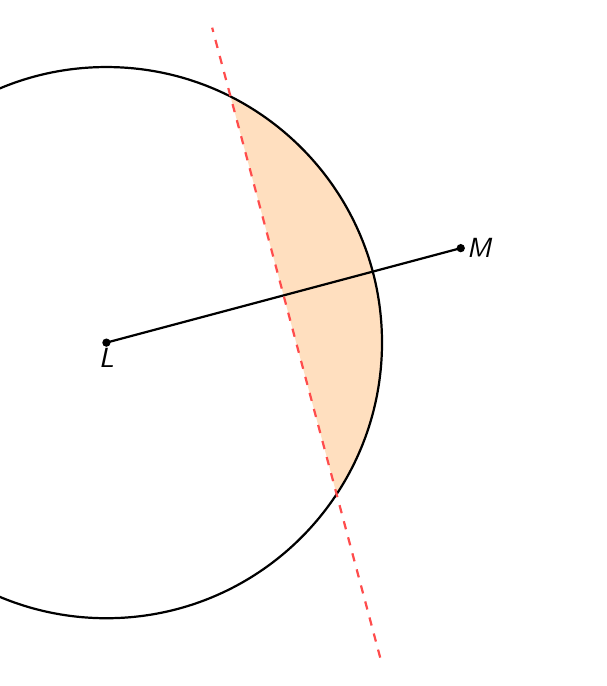
\begin{tikzpicture}[scale=1.0]
  \useasboundingbox (-1,-4) rectangle (6,4);
  \begin{scope}
    \clip (0,0) circle (3.5);
    \fill[orange!25] (3.477,-4) -- (6,-4) -- (6,4) -- (1.343,4) -- cycle;
  \end{scope}
  \draw[given] (0,0) circle (3.5);
  \draw[given] (0,0) -- (4.5,1.2);
  \draw[locus] (3.477,-4) -- (1.343,4);
  \pt{(0,0)}{below}{L}
  \pt{(4.5,1.2)}{right}{M}
\end{tikzpicture}
\end{center}

\s The map shows a farmhouse \(F\) and a straight road. The scale is \(1\)\,cm to \(100\)\,m. The farmer wants to build a straight track from the farmhouse to the road, and wants the track to be as short as possible.
\begin{enumerate}
  \item Use your ruler to draw three different straight tracks from \(F\) to the road. Measure each one.
  \item Construct the perpendicular from \(F\) to the road, and measure it.
  \item Fill in the gap: the shortest distance from a point to a line is along the \underline{\hspace{3.4cm}} from the point to the line.
  \item How long is the shortest track in real life?
\end{enumerate}

\begin{solbox}
(a) Any three straight tracks from \(F\) to the road have lengths greater than the perpendicular distance. For example, they might measure about \(4.5\)\,cm, \(3.8\)\,cm and \(4.2\)\,cm. (b) The perpendicular distance is \(3.5\)\,cm. (c) The shortest distance from a point to a line is along the \textbf{perpendicular} from the point to the line. (d)
\[
3.5\text{ cm}\times 100\text{ m/cm}=350\text{ m}.
\]
\end{solbox}
\ans{(b) \(3.5\)\,cm \qquad (c) perpendicular \qquad (d) \(350\)\,m}

\begin{center}
\begin{tikzpicture}[scale=0.75]
  \useasboundingbox (-0.5,-0.8) rectangle (15,5);
  \draw[given] (0,0) -- (15,0);
  \node[below] at (13.4,0) {road};
  \draw[construction] (5.5,3.5) -- (2,0);
  \draw[construction] (5.5,3.5) -- (7.5,0);
  \draw[construction] (5.5,3.5) -- (11,0);
  \draw[locus] (5.5,3.5) -- (5.5,0);
  \draw (5.5,0) rectangle (5.9,0.4);
  \pt{(5.5,3.5)}{above}{F}
\end{tikzpicture}
\end{center}

\newpage

\section*{D. More loci (Q15--Q18)}

\s The distance from a point to a line is the shortest distance, so it is measured along the perpendicular. In this question we draw the locus of the points that are \(2\)\,cm from the line.
\begin{enumerate}
  \item Construct the perpendicular to the line at \(P\). Mark the two points on your perpendicular that are \(2\)\,cm from \(P\), one on each side of the line.
  \item Do the same at \(Q\).
  \item Use your ruler to draw a straight line through the two points above the line, and another through the two points below the line.
\end{enumerate}

\begin{solbox}
At \(P\), construct the perpendicular and mark \(2\)\,cm above and \(2\)\,cm below the line. Do the same at \(Q\). Joining the two upper points gives a line parallel to the given line, \(2\)\,cm above it. Joining the two lower points gives another parallel line, \(2\)\,cm below it. Together these two parallel lines are the locus.
\end{solbox}

\begin{center}
\begin{tikzpicture}[scale=0.75]
  \useasboundingbox (-0.5,-2.8) rectangle (14.5,2.8);
  \draw[given] (0,0) -- (14,0);
  \draw[locus] (0,2) -- (14,2);
  \draw[locus] (0,-2) -- (14,-2);
  \draw[construction] (3.5,-2.2) -- (3.5,2.2);
  \draw[construction] (10.5,-2.2) -- (10.5,2.2);
  \fill (3.5,2) circle (1.5pt);
  \fill (3.5,-2) circle (1.5pt);
  \fill (10.5,2) circle (1.5pt);
  \fill (10.5,-2) circle (1.5pt);
  \pt{(3.5,0)}{below right}{P}
  \pt{(10.5,0)}{below right}{Q}
\end{tikzpicture}
\end{center}

\s The diagram shows the line segment \(XY\). The dashed lines carry on the line through \(X\) and \(Y\). In this question we draw the locus of the points that are \(2\)\,cm from the line segment \(XY\).
\begin{enumerate}
  \item Construct the perpendicular to the line at \(X\), and the perpendicular to the line at \(Y\).
  \item Mark the points on each perpendicular that are \(2\)\,cm from \(XY\). Join them to draw two line segments that are parallel to \(XY\).
  \item For a point to the left of \(X\), the closest point of the line segment \(XY\) is \(X\) itself. So the points on this side that are \(2\)\,cm from \(XY\) are the points that are \(2\)\,cm from \(X\). Draw them. Do the same to the right of \(Y\).
  \item Priya says, ``The locus of the points that are \(2\)\,cm from \(XY\) is a rectangle.'' Explain why Priya is wrong.
\end{enumerate}

\begin{solbox}
(a) Construct the perpendiculars at \(X\) and \(Y\). (b) Mark \(2\)\,cm above and below \(XY\) at \(X\) and \(Y\), and join corresponding points. This gives two line segments parallel to \(XY\). (c) At the left of \(X\), draw the semicircle of radius \(2\)\,cm centred at \(X\). At the right of \(Y\), draw the semicircle of radius \(2\)\,cm centred at \(Y\). (d) A rectangle would have straight vertical ends. But on a straight vertical side through \(X\), most points are less than \(2\)\,cm from \(X\), so they are not \(2\)\,cm from \(XY\). The true ends are semicircles, and every point on them is exactly \(2\)\,cm from \(X\) or \(Y\).
\end{solbox}

\begin{center}
\begin{tikzpicture}[scale=0.9]
  \useasboundingbox (-3,-3) rectangle (9,3);
  \draw[construction, dashed] (-2.6,0) -- (0,0);
  \draw[construction, dashed] (6,0) -- (8.6,0);
  \draw[given] (0,0) -- (6,0);
  \draw[locus] (0,2) -- (6,2);
  \draw[locus] (0,-2) -- (6,-2);
  \draw[locus] (0,2) arc (90:270:2);
  \draw[locus] (6,2) arc (90:-90:2);
  \pt{(0,0)}{below left}{X}
  \pt{(6,0)}{below right}{Y}
\end{tikzpicture}
\end{center}

\newpage

\s The plan shows a garden. The scale is \(1\)\,cm to \(1\)\,m. A beehive must follow all three rules.
\begin{itemize}
  \item The beehive must be more than \(3\)\,m from the wall of the house.
  \item The beehive must be less than \(4\)\,m from the pond \(P\).
  \item The beehive must be closer to the apple tree \(T\) than to the bench \(B\).
\end{itemize}
Shade the region of the garden where the beehive can go.

\begin{solbox}
Draw the line parallel to the wall, \(3\)\,cm from the wall, and keep the part above it. Draw the circle with centre \(P\) and radius \(4\)\,cm, and keep the inside. Construct the perpendicular bisector of \(TB\), and keep the side containing \(T\). The required region is the part of the garden satisfying all three conditions.

Approximately, along the line \(3\)\,cm from the wall the region runs from about \(2.7\)\,cm to \(5.3\)\,cm from the left-hand fence. Along the top fence it runs from about \(3.6\)\,cm to \(7.5\)\,cm from the left-hand corner. The left boundary is an arc of the circle centred at \(P\), and the right boundary is the perpendicular bisector of \(TB\) until it meets the slanted fence.
\end{solbox}

\begin{center}
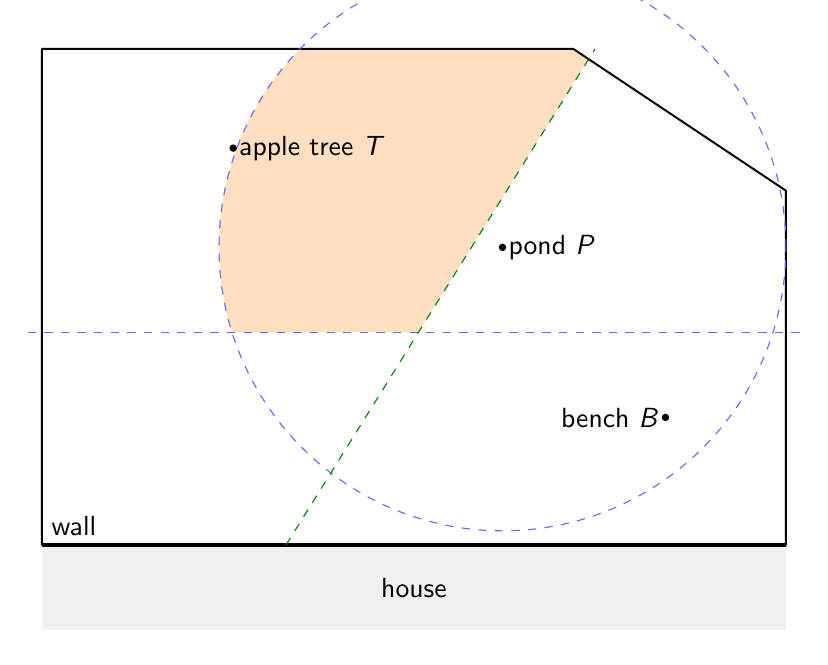
\begin{tikzpicture}[scale=0.9]
  \useasboundingbox (-0.2,-1.3) rectangle (10.7,7.3);
  \fill[black!6] (0,-1.2) rectangle (10.5,0);
  \node at (5.25,-0.6) {house};

  \fill[orange!25]
    (2.685,3) -- (5.314,3) -- (7.716,6.856) -- (7.5,7) -- (3.643,7)
    arc[start angle=135.57,end angle=197.46,radius=4] -- cycle;

  \draw[line width=0.7pt, line join=round]
    (0,0) -- (0,7) -- (7.5,7) -- (10.5,5) -- (10.5,0) -- cycle;
  \draw[line width=1.2pt] (0,0) -- (10.5,0);

  \draw[blue!60, dashed] (-0.2,3) -- (10.7,3);
  \draw[blue!60, dashed] (6.5,4.2) circle (4);
  \draw[green!50!black, dashed] (3.445,0) -- (7.806,7);

  \node[above right] at (0,0) {wall};
  \place{(6.5,4.2)}{right}{pond \(P\)}
  \place{(2.7,5.6)}{right}{apple tree \(T\)}
  \place{(8.8,1.8)}{left}{bench \(B\)}
\end{tikzpicture}
\end{center}

\s Three villages, \(A\), \(B\) and \(C\), are going to share a new phone mast. The mast must be the same distance from all three villages. The scale is \(1\)\,cm to \(2\)\,km.
\begin{enumerate}
  \item Construct the locus of the points that are equidistant from \(A\) and \(B\).
  \item Construct the locus of the points that are equidistant from \(B\) and \(C\).
  \item Mark the point \(M\) where the mast must be built.
  \item Construct the locus of the points that are equidistant from \(A\) and \(C\). What do you notice?
  \item Explain why this happens.
  \item How far is the mast from each village in real life?
\end{enumerate}

\begin{solbox}
(a) The locus equidistant from \(A\) and \(B\) is the perpendicular bisector of \(AB\). (b) The locus equidistant from \(B\) and \(C\) is the perpendicular bisector of \(BC\). (c) The mast \(M\) is the point where these two perpendicular bisectors meet. (d) The perpendicular bisector of \(AC\) also passes through \(M\). (e) Since \(M\) is on the perpendicular bisector of \(AB\), \(MA=MB\). Since \(M\) is on the perpendicular bisector of \(BC\), \(MB=MC\). Hence \(MA=MC\), so \(M\) is equidistant from \(A\) and \(C\), and therefore lies on the perpendicular bisector of \(AC\). (f) On the map \(M\) is \(4\)\,cm from each village. The real distance is
\[
4\times 2=8\text{ km}.
\]
\end{solbox}
\ans{(d) It also passes through \(M\). \qquad (f) \(8\)\,km}

\begin{center}
\begin{tikzpicture}[scale=0.9]
  \useasboundingbox (-5,-5) rectangle (5,5);
  \coordinate (A) at (200:4);
  \coordinate (B) at (320:4);
  \coordinate (C) at (85:4);
  \coordinate (M) at (0,0);
  \coordinate (mAB) at ($(A)!0.5!(B)$);
  \coordinate (mBC) at ($(B)!0.5!(C)$);
  \draw[construction, dashed] (M) circle (4);
  \draw[locus] ($(M)!-2.5!(mAB)$) -- ($(M)!2.5!(mAB)$);
  \draw[locus] ($(M)!-2.5!(mBC)$) -- ($(M)!2.5!(mBC)$);
  \pt{(A)}{left}{A}
  \pt{(B)}{right}{B}
  \pt{(C)}{above}{C}
  \pt{(M)}{below}{M}
\end{tikzpicture}
\end{center}

\newpage

\section*{E. Treasure map (Q19)}

\s A treasure map has these two clues. The scale is \(1\)\,cm to \(10\)\,m.
\begin{itemize}
  \item \textbf{Clue 1:} The treasure is the same distance from the oak tree \(O\) as it is from the well \(W\).
  \item \textbf{Clue 2:} The treasure is \(40\)\,m from the standing stone \(S\).
\end{itemize}
\begin{enumerate}
  \item Use both clues to mark the possible positions of the treasure.
  \item Write a third clue that tells you which of the positions is the treasure. Your clue must describe a locus.
  \item More treasure is buried at the point \(X\). Write some clues that lead to \(X\) and to no other point on the map. Use as few clues as you can, and check your clues by constructing their loci on the map.
\end{enumerate}

\begin{solbox}
(a) Clue 1 gives the perpendicular bisector of \(OW\). Clue 2 gives the circle with centre \(S\) and radius
\[
40\text{ m}\div 10\text{ m/cm}=4\text{ cm}.
\]
These two loci cross at two points, approximately \((6.2,3.9)\) and \((11.1,4.4)\) measured in centimetres from the bottom-left corner of the map. These are the two possible positions of the treasure.

(b) For example: ``The treasure is less than \(50\)\,m from the oak tree \(O\).'' The left-hand position is about \(47\)\,m from \(O\), while the right-hand position is about \(93\)\,m from \(O\). So this clue chooses the left-hand position.

(c) For example, use these clues:
\begin{itemize}
  \item The treasure is about \(80\)\,m from the oak tree \(O\).
  \item The treasure is about \(65\)\,m from the well \(W\).
  \item The treasure is about \(53\)\,m from the standing stone \(S\).
\end{itemize}
On the map these are circles of radii \(8.0\)\,cm, \(6.5\)\,cm and \(5.3\)\,cm. The first two circles meet at \(X\) and at a second point off the left-hand edge of the map; the third circle selects \(X\). If you are allowed to use the edge of the map, the first two clues already lead to \(X\) alone on the map.
\end{solbox}

\begin{center}
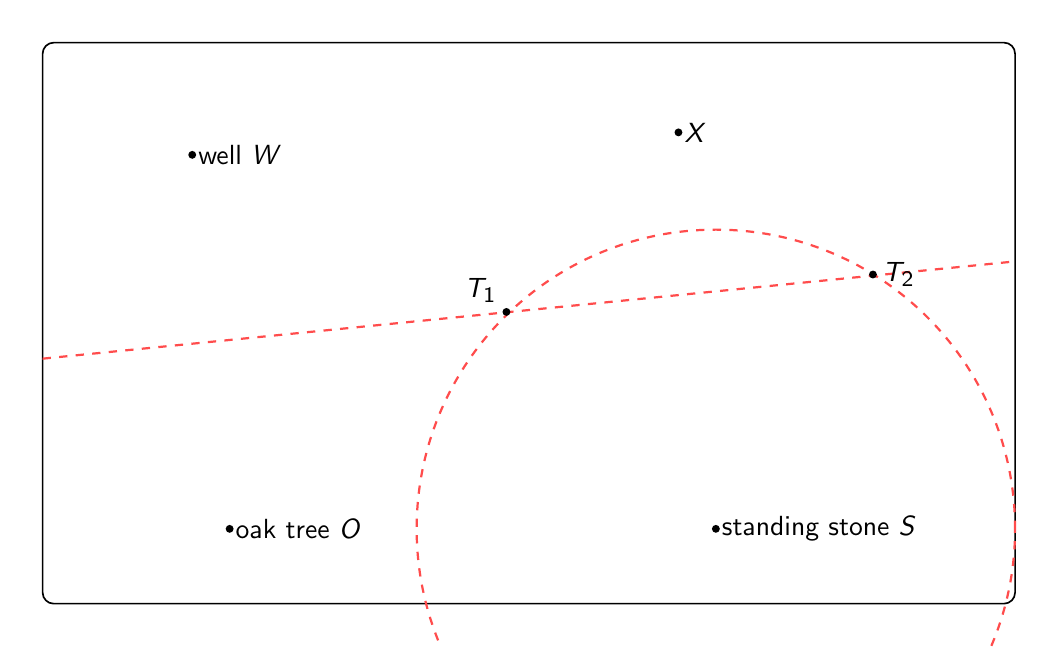
\begin{tikzpicture}[scale=0.95]
  \useasboundingbox (-0.2,-0.2) rectangle (13.2,7.7);
  \draw[line width=0.6pt, rounded corners=4pt] (0,0) rectangle (13,7.5);

  \draw[locus] (0,3.275) -- (13,4.575);
  \draw[locus] (9,1) circle (4);

  \fill (6.2,3.9) circle (1.5pt);
  \node[above left] at (6.2,3.9) {\(T_1\)};
  \fill (11.1,4.4) circle (1.5pt);
  \node[right] at (11.1,4.4) {\(T_2\)};

  \place{(2.5,1)}{right}{oak tree \(O\)}
  \place{(2,6)}{right}{well \(W\)}
  \place{(9,1)}{right}{standing stone \(S\)}
  \pt{(8.5,6.3)}{right}{X}
\end{tikzpicture}
\end{center}

\end{document}